\chapter{Introduction}
\label{chap:intro}

Statistical machine translation (SMT) systems are trained using a large collection of translated
sentence pairs known as a parallel corpus. Common sources of parallel data include
parliament proceedings, books, and news articles.
While this data may be abundant for some language pairs, such as
French/English, it is scarce for most others. In addition, even when parallel
data is available, it often does not match the domain of the data you wish to
translate, which hurts performance \citep{Munteanu05}.

The creation of new parallel corpora can be expensive, especially when bilingual
speakers are rare for the language pair of interest.
In order to acquire more parallel data without costly human annotation,
researchers have looked to multilingual corpora which share some content across languages,
but are not directly translated. Such corpora are referred to as comparable
corpora, and examples include multilingual news feeds \citep{Munteanu05},
Wikipedia articles \citep{Adafre06,Smith10}, and the Web
\citep{Resnik99,Nie99,Chen00}. 
%Most work in extracting parallel sentences from
%these corpora assumes an initial bilingual dictionary or an existing parallel
%corpus.

Comparable corpora is a broad term---\citet{Fung04a} give a more
fine-grained categorization of multilingual corpora:
%TODO: Make sure this is quoted properly
\begin{enumerate}
\item Parallel corpus: A sentence-aligned corpus containing bilingual
translations of the same document.
\item Noisy parallel corpus: A corpus containing non-aligned sentences that are
nevertheless mostly bilingual translations of the same document.
\item Comparable corpus: A corpus of non-aligned and non-translated documents
which are topic-aligned.
\item Quasi-comparable corpus: A multilingual corpus which is not
sentence-aligned, translated, or topic-aligned.
\end{enumerate}
As comparable corpora vary greatly in their structure, different methods for finding
parallel sentences are used in each.

Even corpora which are generally considered as parallel require some amount of
processing to find parallel sentences. The Canadian Hansards, for example,
contains $2:1$ and $1:2$ sentence alignments, and
there may be large insertions or deletions of sentences \citep{Gale93,Chen93}.
Sentence-aligning these corpora does not require existing parallel data or a
bilingual dictionary for the language pair of interest. Instead, the structure
of the documents and the lengths of the sentences are used to determine the
sentence alignment. For comparable corpora which are topic-aligned but not
directly translated, lexical information must be used to determine which
sentence pairs should be aligned \citep{Munteanu05}. When comparable corpora are
not topic-aligned, other signals are exploited to find plausible document
alignments \citep{Resnik03}.

We will examine a representative set of comparable corpora, the Web, Twitter,
and Wikipedia, describe the different signals used to identify parallel data,
and demonstrate how extracted parallel data from these corpora improve SMT
performance across several language pairs and domains. First, we scale up
previous Web mining methods \citep{Resnik03} to several terabytes of data. We
also present a novel mining approach for Twitter, making use of metadata unique
to the microblogging medium. Finally, we introduce a new sentence alignment
model for mining parallel data from Wikipedia which takes advantage of its
fine-grained topic alignment.

\section{What counts as parallel?}
This work is centered around finding parallel data---bilingual sentence pairs
which convey the same meaning. Unfortunately, it is extremely difficult, if not
impossible, to determine whether or not two sentences in different languages
have the same meaning. One language may contain gender markings that the other
does not, or the connotation of a word may be difficult to express in another
language. Examples of this problem are explored in depth by \citet{Kay97}. 
Even ignoring the cross-lingual issues, comparing the meaning of two sentences
in the same language is still quite difficult---SMT evaluation metrics
\citep{Papineni02,Banerjee05,Snover06} must address this problem.

When directly evaluating methods for finding parallel data (intrinsic
evaluation), we need some criteria for determining whether or not a bilingual
sentence pair is parallel. This is easy if we use parallel data, but
it is preferable to evaluate our methods on the same corpora that we are
extracting data from. When designing the criteria for judging parallel
sentences, we focus on our goal: improving SMT performance. If a sentence pair
is likely to improve performance when added to our SMT system's training data,
we would like to extract it. The details of our annotation criteria can be found
in Chapter \ref{chap:supervised}, but in all cases they are motivated by SMT
performance. To understand what will influence performance, we need to
understand modern SMT systems.

\section{Statistical Machine Translation}
While machine translation has been around in some form for many decades
\citep{Locke55}, statistical machine translation began with the work of
\citet{Brown93}. SMT systems have evolved since then, most notably moving from
word-based systems to phrase-based \citep{Koehn03}. Several newer systems have
been developed, focusing mostly on incorporating syntax into the translation
model \citep{Chiang05,Quirk05,Liu06,Galley06}. These systems all share some key
characteristics in how they use parallel data:

\begin{enumerate}
\item A large collection of parallel sentences are used as training data.
\item These sentence pairs are word-aligned using IBM-Models \citep{Brown93}
and/or hidden Markov models \citep{Vogel96}.
\item Pairs of phrases, or other multi-word units, are extracted from the
word-aligned sentence pairs to form a translation model.
\item A language model is created from large amounts of monolingual data in the
``target'' language (the language which text is translated into). This includes
the target side of the parallel training data.
\end{enumerate}

There are additional details in each model, but the main effects of adding new
parallel data are additional inputs to the translation and language models.

\section{Evaluation Pipeline}
Our evaluation setup is identical across chapters---we start with {\em initial}
data that includes some standard parallel and monolingual corpora commonly used for 
translation. We also have {\em extracted} parallel data that we find in a comparable
corpus. Table \ref{tab:exp_setup} describes how we use this data to measure SMT
improvements:

\begin{table}
\begin{center}
\begin{tabular}{|c||c|c|}
\hline
& Parallel & Monolingual \\
\hline
Baseline & Initial & Initial + Extracted \\
\hline
Experimental & Initial + Extracted & Initial + Extracted \\
\hline
\end{tabular}
\end{center}
\label{tab:exp_setup}
\caption{Parallel and monolingual data used in our SMT experiments.}
\end{table}

In both the baseline and experimental conditions, we include the target side of
the extracted parallel sentences in the monolingual training data. We do this to
ensure that any increase in performance is coming from the parallel data. It
would be simple to add monolingual text from a comparable corpus to an SMT
system.

In all experiments, the BLEU metric \citep{Papineni02} is used to evaluate SMT
performance. The initial data, test sets, and other details vary by
experiment.

\section{Sentence Alignment}
In this section, we will describe our task and notation.
We will view both parallel corpora alignment and the extraction of parallel
sentences from comparable corpora as an alignment task. In either type of
alignment we are given a set of bilingual document pairs in {\em source} and {\em
target} languages. When performing parallel corpora alignment, these document
pairs will correspond to each other very strongly, while in the case of
comparable corpora, some these document pairs may contain no parallel sentences.
\citet{Munteanu05} take their document pairs from news stories published at
roughly the same time, while \citet{Adafre06,Smith10} use entries from
Wikipedia that are on the same topic (Figure \ref{fig:wiki} gives and example).
The task of finding comparable document pairs is not addressed in this work.

\begin{figure*}[ht]
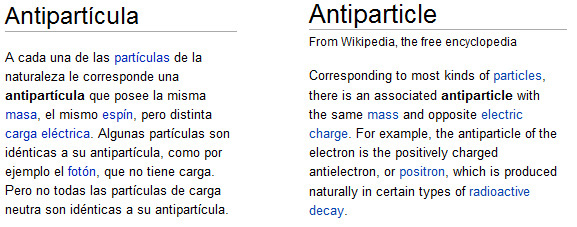
\includegraphics[width=\textwidth]{images/wiki.jpg}
\caption{An example of a Spanish/English document pair from Wikipedia.}
\label{fig:wiki}
\end{figure*}

Each document pair contains a sequence of source sentences (denoted by ${\bf
S}$) and target sentences (denoted by ${\bf T}$). Individual source and target
sentences are referred to by $S$ and $T$ respectively. Similarly, we refer to
the words within source and target sentences with the lowercase $s$ and $t$. We
borrow the notation of \citep{Och03} for describing alignments between sentences
as subsets of the Cartesian product of sentence positions. Sentence alignments
are referred to with the uppercase $A$, and word alignments with the lowercase
$a$.

The goal of sentence alignment is to identify which sentence pairs in the
bilingual document pairs are parallel. We view this as a retrieval task for
parallel sentence pairs, and so when annotated sentence alignments are present,
we can compute precision, recall, and F-measure.
